% Provenance (never printed): cycle 4 SVT, "La planete Terre, l'environnement
% et l'action humaine": the relief as a balance between uplift and erosion;
% landforms of the wind, the sea and dissolution; reading a landscape; see
% sources/book1/PROVENANCE.md. Book 1, grade 9, chapter 4.
% Vocabulary guard: owns uplift, dune, cliff, beach and spit (with longshore
% drift), karst (with cave and sinkhole). Landscape and landform are g1's;
% weathering, erosion, deposition, meander and delta are g5's; relief is
% g4's; plates and mountain building are g7's; U-shaped valley and moraine
% are g8's; limestone and the acid test are g6's; acids are the chemistry
% books' (recalled in prose). Contour lines are g9.5's (not used here).
% "Normal fault" and the destruction of mountains are Book 2's.
\chapter{Bentuk Lahan}\label{ch:g9:landforms}

Di \omterm{def:g1:landscapes-around-us:water}{pesisir} selatan Inggris, \omterm{def:g9:landforms:cliff}{tebing-tebing} putih Seven Sisters jatuh tegak
lurus ke \omterm{def:g2:water-on-earth:ocean}{laut}. Pada tahun biasa, \omterm{def:g9:landforms:cliff}{tebing-tebing} itu kehilangan sampai satu
meter. Pada musim dingin tahun 2014, \omterm{def:g5:natural-hazards:storm}{badai-badai} mengambil dari \omterm{def:g9:landforms:cliff}{tebing} di
Birling Gap sebanyak yang biasanya hilang dalam tujuh tahun, hanya dalam
dua bulan. Kapur pada \omterm{def:g9:landforms:cliff}{tebing-tebing} ini dahulu adalah \omterm{def:g3:stones-pebbles-sand:sand}{lumpur} di dasar
sebuah \omterm{def:g2:water-on-earth:ocean}{laut}, yang tersusun atas lempeng-lempeng kecil dari ganggang
mikroskopis yang hidup di airnya. Sekarang kapur itu berdiri sebagai
dinding \omterm{def:g3:stones-pebbles-sand:rock}{batuan} putih yang dikikis ombak sedikit demi sedikit setiap tahun.
Mengapa daratan mempunyai bentuk-bentuk seperti yang dimilikinya, dan
mengapa sebagian bentuk itu berubah begitu cepat?
% ledger: nt:birling-2014, sdnp:birling, nasa:coccoliths

\begin{omfigure}
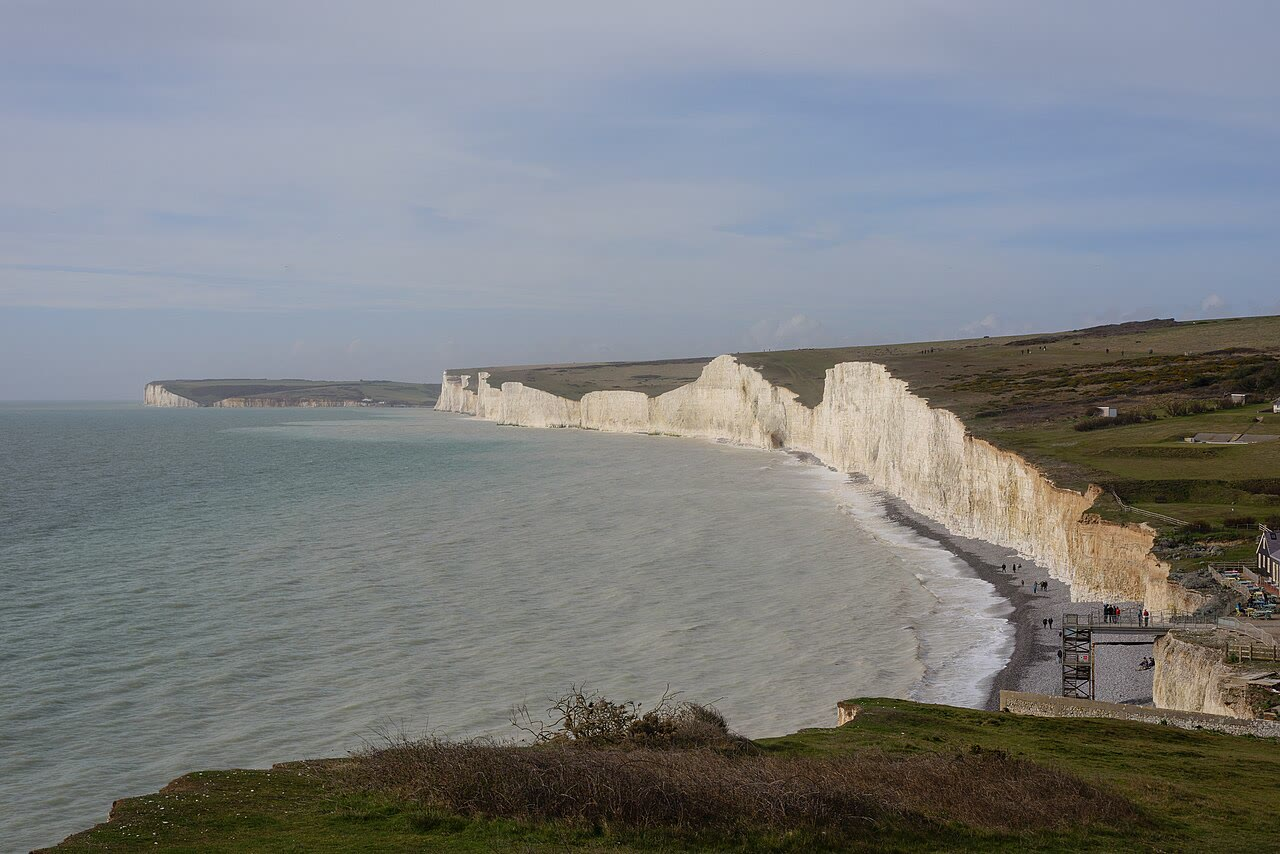
\includegraphics[width=\linewidth]{images/book1/g9-seven-sisters.jpg}

{\small Seven Sisters, \omterm{def:g9:landforms:cliff}{tebing} kapur di \omterm{def:g1:landscapes-around-us:water}{pesisir} East Sussex (Inggris),
dengan rumah-rumah Birling Gap di latar depan. \omterm{def:g9:landforms:cliff}{Tebing-tebing} itu dikikis
mundur oleh \omterm{def:g2:water-on-earth:ocean}{laut}, dan runtuhan batu dapat terjadi kapan saja. Di kakinya
terbentang \omterm{def:g9:landforms:beach}{gisik} berkerikil. Foto Arild Vågen, 2017 (CC BY-SA 4.0, melalui
Wikimedia Commons).}
% ledger: commons:seven-sisters, sdnp:birling
\label{fig:g9:landforms:seven-sisters}
\end{omfigure}

\begin{recall}
\emph{\omterm{def:g1:landscapes-around-us:landform}{Bentuk lahan}}, yang juga disebut \omterm{def:g1:landscapes-around-us:landform}{bentuk muka bumi}, adalah salah satu
bentuk daratan: \omterm{def:g1:landscapes-around-us:landform}{bukit}, \omterm{def:g1:landscapes-around-us:landform}{lembah}, \omterm{def:g1:landscapes-around-us:landform}{dataran}, \omterm{def:g9:landforms:cliff}{tebing}
(\cref{ch:g1:landscapes-around-us}). \omterm{def:g4:world-physical-map:relief}{Relief} adalah bentuk
daratan dalam hal \omterm{def:g4:world-physical-map:altitude}{ketinggiannya} (\cref{ch:g4:world-physical-map}).
\omterm{def:g5:water-shapes-the-land:weathering}{Pelapukan} memecah \omterm{def:g3:stones-pebbles-sand:rock}{batuan}, \omterm{def:g5:water-shapes-the-land:erosion}{erosi} mengikisnya dan membawanya pergi, dan
\omterm{def:g5:water-shapes-the-land:deposition}{pengendapan} meletakkannya di tempat lain
(\cref{ch:g5:water-shapes-the-land}). \omterm{def:g7:plate-tectonics:plate}{Lempeng-lempeng} mendorong naik
rangkaian \omterm{def:g4:world-physical-map:range}{pegunungan} di tempat keduanya bertumbukan
(\cref{ch:g7:plate-tectonics}); \omterm{def:g8:ice-on-earth:glacier}{gletser} mengukir \omterm{def:g8:ice-on-earth:glacial-landforms}{lembah berbentuk U}
(\cref{ch:g8:ice-on-earth}); batu kapur berbuih jika ditetesi asam encer
(\cref{ch:g6:rocks-and-minerals}). Dalam kimia, kamu belajar bahwa asam
menyerang batu kapur dan melepaskan karbon dioksida.
\end{recall}

\section{Relief: keseimbangan antara pengangkatan dan erosi}

Dua macam gaya membentuk \omterm{def:g4:world-physical-map:relief}{relief}. Dari dalam, gerakan \omterm{def:g7:plate-tectonics:plate}{lempeng-lempeng}
mengangkat permukaan tanah. Dari luar, air, es, angin, dan \omterm{def:g2:water-on-earth:ocean}{laut}
mengikisnya.

\begin{definition}[Pengangkatan]\label{def:g9:landforms:uplift}
Yang disebut \emph{pengangkatan}\index{pengangkatan} adalah naiknya
\omterm{def:g3:stones-pebbles-sand:rock}{batuan} dan permukaan tanah suatu wilayah secara perlahan, yang digerakkan
oleh gaya-gaya di dalam Bumi, misalnya tumbukan dua \omterm{def:g7:plate-tectonics:plate}{lempeng}.
\end{definition}

\omterm{def:g9:landforms:uplift}{Pengangkatan} berlangsung lambat pada skala hidup manusia, tetapi cepat
pada skala Bumi. India bertumbukan dengan Asia sekitar 50~juta tahun yang
lalu, dan \omterm{def:g1:landscapes-around-us:landform}{Dataran} Tinggi Tibet, di belakang Himalaya, memperoleh sebagian
besar \omterm{def:g4:world-physical-map:altitude}{ketinggiannya}, sekitar \qty{4600}{m}, dalam 10~juta tahun terakhir.
Rata-rata, itu berarti
$4600 \div 10^7 = 4.6 \times 10^{-4}$~m, atau sekitar \qty{0.5}{mm}
setahun: lebih tipis daripada tebal kuku jari, tetapi berlangsung terus
selama jutaan tahun.
% ledger: usgs:himalaya (rate computed in figdata/grade-9/cliff_retreat.py, tibet_rate_mm_yr)

Begitu tanah naik, \omterm{def:g5:water-shapes-the-land:erosion}{erosi} menyerangnya. Makin tinggi dan makin curam
daratan, makin cepat \omterm{def:g1:landscapes-around-us:water}{sungai}, \omterm{def:g8:ice-on-earth:glacier}{gletser}, dan runtuhan batu mengangkut \omterm{def:g3:stones-pebbles-sand:rock}{batuan}
pergi. \omterm{def:g4:world-physical-map:altitude}{Ketinggian} suatu rangkaian \omterm{def:g4:world-physical-map:range}{pegunungan} pada saat mana pun adalah
hasil sebuah pertandingan: apa yang dinaikkan oleh \omterm{def:g9:landforms:uplift}{pengangkatan}, dikurangi
apa yang diambil oleh \omterm{def:g5:water-shapes-the-land:erosion}{erosi}.

\begin{omfigure}
\begin{tikzpicture}[font=\footnotesize, >={Stealth[length=2mm]}]
  % panel 1: uplift faster than erosion
  \begin{scope}
    \fill[black!13] (0,0) -- (0.5,0) .. controls (1.1,1.0) and (1.5,2.0) .. (1.8,2.2)
      .. controls (2.1,2.0) and (2.5,1.0) .. (3.1,0) -- (3.6,0) -- (3.6,-0.5) -- (0,-0.5) -- cycle;
    \draw[black!60] (0,0) -- (0.5,0) .. controls (1.1,1.0) and (1.5,2.0) .. (1.8,2.2)
      .. controls (2.1,2.0) and (2.5,1.0) .. (3.1,0) -- (3.6,0);
    \draw[black!60, dashed] (0.7,0) .. controls (1.2,0.8) and (1.5,1.5) .. (1.8,1.6)
      .. controls (2.1,1.5) and (2.4,0.8) .. (2.9,0);
    \foreach \x in {1.2,1.8,2.4} \draw[->, omWarm, line width=1.4pt] (\x,-0.45) -- ++(0,1.0);
    \draw[->, omRiver, thick] (2.15,1.6) -- ++(0.35,-0.3);
    \node[align=center, anchor=north] at (1.8,-0.6) {pengangkatan lebih\\cepat daripada erosi:\\relief naik};
  \end{scope}
  % panel 2: uplift equals erosion
  \begin{scope}[xshift=4.4cm]
    \fill[black!13] (0,0) -- (0.5,0) .. controls (1.1,1.0) and (1.5,1.8) .. (1.8,1.9)
      .. controls (2.1,1.8) and (2.5,1.0) .. (3.1,0) -- (3.6,0) -- (3.6,-0.5) -- (0,-0.5) -- cycle;
    \draw[black!60] (0,0) -- (0.5,0) .. controls (1.1,1.0) and (1.5,1.8) .. (1.8,1.9)
      .. controls (2.1,1.8) and (2.5,1.0) .. (3.1,0) -- (3.6,0);
    \foreach \x in {1.2,1.8,2.4} \draw[->, omWarm, line width=1.4pt] (\x,-0.45) -- ++(0,0.6);
    \draw[->, omRiver, thick] (2.05,1.6) -- ++(0.55,-0.5);
    \draw[->, omRiver, thick] (1.55,1.6) -- ++(-0.55,-0.5);
    \node[align=center, anchor=north] at (1.8,-0.6) {pengangkatan sama\\dengan erosi:\\ketinggian tetap};
  \end{scope}
  % panel 3: no more uplift
  \begin{scope}[xshift=8.8cm]
    \fill[black!13] (0,0) -- (0.4,0) .. controls (1.1,0.5) and (1.5,0.95) .. (1.8,1.0)
      .. controls (2.1,0.95) and (2.5,0.5) .. (3.2,0) -- (3.6,0) -- (3.6,-0.5) -- (0,-0.5) -- cycle;
    \draw[black!60] (0,0) -- (0.4,0) .. controls (1.1,0.5) and (1.5,0.95) .. (1.8,1.0)
      .. controls (2.1,0.95) and (2.5,0.5) .. (3.2,0) -- (3.6,0);
    \draw[black!60, dashed] (0.5,0) .. controls (1.1,1.0) and (1.5,1.8) .. (1.8,1.9)
      .. controls (2.1,1.8) and (2.5,1.0) .. (3.1,0);
    \draw[->, omRiver, thick] (2.05,0.95) -- ++(0.55,-0.5);
    \draw[->, omRiver, thick] (1.55,0.95) -- ++(-0.55,-0.5);
    \node[align=center, anchor=north] at (1.8,-0.6) {pengangkatan berhenti:\\erosi menurunkan\\relief};
  \end{scope}
  % key
  \draw[->, omWarm, line width=1.4pt] (13.2,1.2) -- ++(0,0.6) node[right, black] {pengangkatan};
  \draw[->, omRiver, thick] (13.2,0.7) -- ++(0.35,-0.3) node[right, black] {erosi};
  \draw[black!60, dashed] (13.1,-0.1) -- ++(0.5,0) node[right, black] {profil sebelumnya};
\end{tikzpicture}

{\small \omterm{def:g4:world-physical-map:relief}{Relief} sebagai keseimbangan (sketsa, tidak berskala). \omterm{def:g9:landforms:uplift}{Pengangkatan}
menaikkan \omterm{def:g3:stones-pebbles-sand:rock}{batuan}; \omterm{def:g5:water-shapes-the-land:erosion}{erosi} mengangkutnya pergi ke \omterm{def:g1:landscapes-around-us:landform}{lembah} dan ke \omterm{def:g2:water-on-earth:ocean}{laut}. Suatu
rangkaian \omterm{def:g4:world-physical-map:range}{pegunungan} terus tumbuh selama \omterm{def:g9:landforms:uplift}{pengangkatan} menang; ketika
\omterm{def:g7:plate-tectonics:plate}{lempeng-lempeng} berhenti mendorong, \omterm{def:g5:water-shapes-the-land:erosion}{erosi} perlahan-lahan mengikisnya
sampai menjadi perbukitan.}
\label{fig:g9:landforms:balance}
\end{omfigure}

\omterm{def:g1:landscapes-around-us:water}{Sungai} (\cref{ch:g5:water-shapes-the-land}) dan \omterm{def:g8:ice-on-earth:glacier}{gletser}
(\cref{ch:g8:ice-on-earth}) adalah pemahat utama \omterm{def:g4:world-physical-map:range}{pegunungan}. Bagian
selanjutnya bab ini mengikuti tiga tenaga lain, yang masing-masing
membuat \omterm{def:g1:landscapes-around-us:landform}{bentuk lahannya} sendiri: angin, \omterm{def:g2:water-on-earth:ocean}{laut}, dan air yang melarutkan
\omterm{def:g3:stones-pebbles-sand:rock}{batuan}.

\section{Bentuk lahan buatan angin: gumuk pasir}

Di tempat tumbuhan jarang, \omterm{def:g3:stones-pebbles-sand:sand}{pasir} lepas berlimpah, dan angin kencang,
angin dapat memungut \omterm{def:g3:stones-pebbles-sand:sand}{pasir} dan menimbunnya menjadi \omterm{def:g1:landscapes-around-us:landform}{bukit}: di \omterm{def:g5:weather-and-climate:desert}{gurun}, dan di
belakang pantai berpasir.
% ledger: nps:aeolian

\begin{definition}[Gumuk pasir]\label{def:g9:landforms:dune}
Yang disebut \emph{gumuk pasir}\index{gumuk pasir} adalah gundukan atau
pematang \omterm{def:g3:stones-pebbles-sand:sand}{pasir} lepas yang ditimbun oleh angin. Lerengnya yang menghadap
angin panjang dan landai; sisi seberangnya, yaitu \emph{lereng
luncur}\index{lereng luncur}, pendek dan curam.
\end{definition}
% ledger: nps:aeolian, nmt:barchan

\omterm{def:g9:landforms:dune}{Gumuk pasir} bergerak. Angin menggulirkan dan melontarkan butir-butir \omterm{def:g3:stones-pebbles-sand:sand}{pasir}
menaiki lereng yang landai; di puncak, butir-butir itu menumpuk sampai
timbunannya menjadi terlalu curam, lalu longsoran kecil \omterm{def:g3:stones-pebbles-sand:sand}{pasir} meluncur
menuruni \omterm{def:g9:landforms:dune}{lereng luncur}. Butir demi butir, \omterm{def:g3:stones-pebbles-sand:sand}{pasir} diambil dari sisi yang
menghadap angin dan diletakkan di sisi seberangnya, dan seluruh \omterm{def:g9:landforms:dune}{gumuk} itu
merayap searah angin tanpa pernah terangkat. \omterm{def:g9:landforms:dune}{Gumuk pasir} jarang berdiri
sendirian: \omterm{def:g9:landforms:dune}{gumuk-gumuk} itu menutupi padang yang luas.
% ledger: nmt:barchan, nps:aeolian

Di tempat angin selalu bertiup dari arah yang sama dan \omterm{def:g3:stones-pebbles-sand:sand}{pasirnya} tidak
terlalu banyak, \omterm{def:g9:landforms:dune}{gumuk pasir} berbentuk bulan sabit, yang disebut
\emph{barkan}: hidungnya yang bundar menghadap angin dan kedua tanduknya
menunjuk searah angin. Tanduk-tanduknya mengandung lebih sedikit \omterm{def:g3:stones-pebbles-sand:sand}{pasir}
daripada bagian tengahnya, sehingga bergerak lebih cepat dan memanjang
mendahului \omterm{def:g9:landforms:dune}{gumuknya}.
% ledger: nmt:barchan

\begin{omfigure}
\begin{tikzpicture}[font=\footnotesize, >={Stealth[length=2mm]}]
  % plan view
  \fill[yellow!25!orange!20] (3.4,1.3) .. controls (1.0,1.3) and (0.2,0.6) .. (0.2,0)
     .. controls (0.2,-0.6) and (1.0,-1.3) .. (3.4,-1.3)
     .. controls (2.4,-0.9) and (1.8,-0.5) .. (1.8,0)
     .. controls (1.8,0.5) and (2.4,0.9) .. (3.4,1.3) -- cycle;
  \fill[orange!45] (3.4,1.3) .. controls (2.4,0.9) and (1.8,0.5) .. (1.8,0)
     .. controls (1.8,-0.5) and (2.4,-0.9) .. (3.4,-1.3)
     .. controls (2.1,-0.8) and (1.45,-0.45) .. (1.45,0)
     .. controls (1.45,0.45) and (2.1,0.8) .. (3.4,1.3) -- cycle;
  \draw[black!60] (3.4,1.3) .. controls (1.0,1.3) and (0.2,0.6) .. (0.2,0)
     .. controls (0.2,-0.6) and (1.0,-1.3) .. (3.4,-1.3)
     .. controls (2.4,-0.9) and (1.8,-0.5) .. (1.8,0)
     .. controls (1.8,0.5) and (2.4,0.9) .. (3.4,1.3);
  \draw[black, thick] (3.4,1.3) .. controls (2.1,0.8) and (1.45,0.45) .. (1.45,0)
     .. controls (1.45,-0.45) and (2.1,-0.8) .. (3.4,-1.3);
  \foreach \y in {-0.8,0,0.8} \draw[->, omRiver, thick] (-1.3,\y) -- ++(1.1,0);
  \node[above] at (-0.75,0.85) {angin};
  \node[anchor=west] at (3.5,1.35) {tanduk};
  \node[anchor=west] at (3.5,-1.35) {tanduk};
  \draw[black!70] (1.75,0.25) -- (2.9,0.35) node[anchor=west, align=left, black] {lereng luncur\\(curam)};
  \draw[black!70] (0.75,-0.2) -- (0.6,-1.6) node[anchor=north, align=center, black] {lereng\\hadap angin\\(landai)};
  \draw[black!70] (1.47,-0.3) -- (2.4,-1.75) node[anchor=north, black] {puncak};
  \node[anchor=south, font=\footnotesize\bfseries] at (1.4,1.6) {dilihat dari atas};
  % profile
  \begin{scope}[xshift=7.2cm, yshift=-0.8cm]
    \draw[black!60] (-0.4,0) -- (5.6,0);
    \fill[yellow!25!orange!20] (0,0) -- (3.0,1.2) -- (3.6,0) -- cycle;
    \draw[black!70] (0,0) -- (3.0,1.2) -- (3.6,0);
    \fill[orange!45] (3.0,1.2) -- (3.6,0) -- (3.3,0) -- cycle;
    \draw[black!50, dashed] (0.8,0) -- (3.8,1.2) -- (4.4,0);
    \draw[->, black!70] (0.5,0.35) .. controls (0.75,0.65) .. (1.0,0.45);
    \draw[->, black!70] (1.0,0.55) .. controls (1.25,0.85) .. (1.5,0.65);
    \draw[->, black!70] (1.5,0.75) .. controls (1.75,1.05) .. (2.0,0.85);
    \draw[->, black!70] (2.0,0.95) .. controls (2.25,1.25) .. (2.5,1.05);
    \draw[->, thick, black!80] (3.15,1.05) -- (3.45,0.35);
    \foreach \y in {1.6,2.1} \draw[->, omRiver, thick] (-0.8,\y) -- ++(1.1,0);
    \node[above] at (-0.25,2.1) {angin};
    \draw[->, thick] (4.5,0.6) -- ++(0.7,0) node[right, align=left] {gumuk\\bergerak};
    \node[align=center, anchor=north] at (1.2,-0.1) {butir-butir\\melompat naik di\\lereng yang landai};
    \node[align=center, anchor=north west] at (2.9,-0.1) {lalu meluncur\\turun di\\lereng luncur};
    \node[anchor=south, font=\footnotesize\bfseries] at (2.2,2.3) {dilihat dari samping};
  \end{scope}
\end{tikzpicture}

{\small \omterm{def:g9:landforms:dune}{Gumuk pasir} bulan sabit, atau barkan (sketsa). Dilihat dari atas,
tanduk-tanduknya menunjuk searah angin. Dilihat dari samping, butir-butir
\omterm{def:g3:stones-pebbles-sand:sand}{pasir} mendaki lereng hadap angin yang landai dan meluncur turun di \omterm{def:g9:landforms:dune}{lereng
luncur} yang curam: \omterm{def:g9:landforms:dune}{gumuk} itu bergerak searah angin (garis putus-putus:
\omterm{def:g9:landforms:dune}{gumuk} itu beberapa waktu kemudian).}
% ledger: nmt:barchan, nps:aeolian
\label{fig:g9:landforms:barchan}
\end{omfigure}

Seberapa cepat? Di padang \omterm{def:g9:landforms:dune}{gumuk} gipsum White Sands, di New Mexico,
\omterm{def:g9:landforms:dune}{gumuk-gumuk} kecil yang terbentuk di tepi hulu anginnya, setinggi beberapa
meter, bergerak sampai \qty{6}{m} setahun; sedikit lebih jauh, setelah
tumbuh setinggi 6 sampai \qty{10}{m}, \omterm{def:g9:landforms:dune}{gumuk-gumuk} itu bergerak sekitar
\qty{3}{m} setahun. Makin banyak \omterm{def:g3:stones-pebbles-sand:sand}{pasir} yang dikandung sebuah \omterm{def:g9:landforms:dune}{gumuk}, makin
lambat gerakannya. Barkan yang didorong angin kencang dapat berpindah lebih
dari \qty{100}{m} dalam setahun, cukup untuk mengubur jalan atau ladang.
% ledger: nps:whsa-migration, nmt:barchan

\begin{omfigure}
\begin{minipage}[c]{0.5\linewidth}\centering
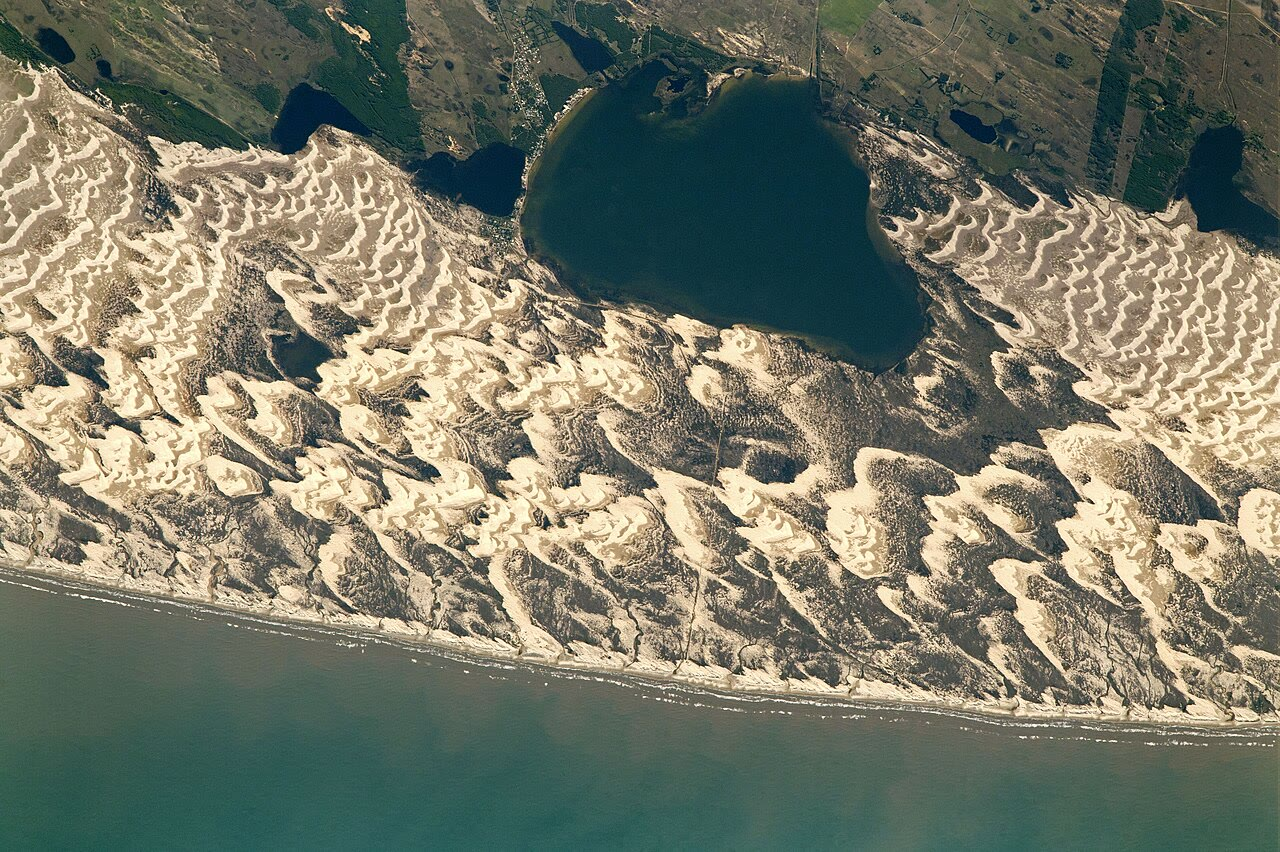
\includegraphics[width=\linewidth]{images/book1/g9-barchans.jpg}
\end{minipage}\hfill
\begin{minipage}[c]{0.46\linewidth}\raggedright
{\small \omterm{def:g9:landforms:dune}{Gumuk-gumuk} \omterm{def:g3:stones-pebbles-sand:sand}{pasir} berbentuk bulan sabit di \omterm{def:g1:landscapes-around-us:water}{pesisir} Atlantik
Brasil selatan, yang dipotret oleh seorang astronaut dari Stasiun
Antariksa Internasional pada tahun 2017. \omterm{def:g1:landscapes-around-us:water}{Danau} yang gelap, Lagoa dos
Barros, panjangnya sekitar \qty{4.5}{km}. \omterm{def:g3:stones-pebbles-sand:sand}{Pasirnya} berasal dari pantai, di
bagian bawah foto. NASA (domain publik, melalui Wikimedia Commons).}
\end{minipage}
% ledger: commons:iss-barchans
\label{fig:g9:landforms:barchans-photo}
\end{omfigure}

Di \omterm{def:g1:landscapes-around-us:water}{pesisir}, deretan \omterm{def:g9:landforms:dune}{gumuk pasir} di belakang pantai melindungi daratan di
belakangnya dari ombak \omterm{def:g5:natural-hazards:storm}{badai}. Tumbuhan yang tumbuh di \omterm{def:g9:landforms:dune}{gumuk pasir} menahan
\omterm{def:g3:stones-pebbles-sand:sand}{pasir} dengan akar-akarnya: di tempat tumbuhan itu terinjak-injak atau
dibabat, angin kembali menerbangkan \omterm{def:g3:stones-pebbles-sand:sand}{pasirnya}.
% ledger: nps:aeolian

\section{Bentuk lahan buatan laut}

\subsection{Tebing}

\begin{definition}[Tebing]\label{def:g9:landforms:cliff}
Yang disebut \emph{tebing}\index{tebing} adalah permukaan \omterm{def:g3:stones-pebbles-sand:rock}{batuan} yang
curam atau tegak lurus. Di \omterm{def:g1:landscapes-around-us:water}{pesisir}, tebing dipahat oleh ombak, yang
menyerang kakinya dan membuatnya mundur ke arah daratan.
\end{definition}

Ombak melemparkan air, \omterm{def:g3:stones-pebbles-sand:sand}{pasir}, dan \omterm{def:g3:stones-pebbles-sand:pebble}{kerikil} ke kaki \omterm{def:g9:landforms:cliff}{tebing}. Sedikit demi
sedikit, ombak memahat sebuah ceruk di dasarnya, yaitu \emph{takik}, di
antara ketinggian air surut dan air pasang. \omterm{def:g3:stones-pebbles-sand:rock}{Batuan} di atasnya menggantung;
\omterm{def:g4:clouds-rain-snow:precipitation}{hujan} dan embun beku melemahkannya lagi. Suatu hari, bagian yang
menggantung itu runtuh. Ombak memecah bongkah-bongkah yang jatuh dan
mengangkutnya pergi, lalu serangan dimulai lagi pada permukaan yang baru,
sedikit lebih jauh ke arah daratan. Di belakangnya, \omterm{def:g9:landforms:cliff}{tebing} itu
meninggalkan paparan \omterm{def:g3:stones-pebbles-sand:rock}{batuan} yang datar, yaitu \emph{dataran
abrasi}\index{dataran abrasi}, yang muncul saat air surut.
% ledger: nt:birling-2014, sdnp:birling

\omterm{def:g3:stones-pebbles-sand:rock}{Batuan} yang lunak mundur paling cepat. Di Birling Gap, \omterm{def:g9:landforms:cliff}{tebing} kapur
kehilangan sampai sekitar satu meter setahun; tetapi mundurnya terjadi
dengan lompatan, satu runtuhan setiap kali, dan musim dingin yang penuh
\omterm{def:g5:natural-hazards:storm}{badai} dapat mengambil mundurnya bertahun-tahun sekaligus. Pada tahun
1999, mercusuar tua Belle Tout, yang dibangun pada tahun 1832 di atas
\omterm{def:g9:landforms:cliff}{tebing} di dekatnya, dipindahkan \qty{17}{m} menjauhi tepi \omterm{def:g9:landforms:cliff}{tebing}, utuh
dalam satu bagian, karena \omterm{def:g9:landforms:cliff}{tebing} itu sudah terlalu dekat.
% ledger: sdnp:birling, nt:birling-2014

\begin{omfigure}
\begin{tikzpicture}[font=\footnotesize, >={Stealth[length=2mm]}]
  % panel 1: the notch
  \begin{scope}
    \fill[omSea!45] (0,-0.1) rectangle (1.8,0.75);
    \fill[omSea!45] (1.8,0.35) -- (2.25,0.55) -- (1.8,0.95) -- cycle;
    \fill[black!8] (1.6,-0.1) -- (1.8,0.25) -- (1.8,0.35) -- (2.25,0.55) -- (1.8,0.95) -- (1.8,2.4) -- (3.6,2.4) -- (3.6,-0.6) -- (0,-0.6) -- (0,-0.1) -- cycle;
    \draw[black!70] (0,-0.1) -- (1.6,-0.1) -- (1.8,0.25) -- (1.8,0.35) -- (2.25,0.55) -- (1.8,0.95) -- (1.8,2.4) -- (3.6,2.4);
    \foreach \y in {0.8,1.3,1.8} \draw[black!25] (1.8,\y) -- (3.6,\y);
    \fill[green!35!black!50] (1.8,2.4) rectangle (3.6,2.5);
    \draw[->, omSea!80!black, thick] (0.4,0.6) -- (1.6,0.6);
    \node[anchor=south, align=center] at (0.9,0.8) {ombak};
    \draw[black!70] (2.15,0.55) -- (2.9,1.0) node[anchor=west, fill=white, inner sep=1pt] {takik};
    \node[anchor=north, align=center] at (1.8,-0.7) {1. ombak memahat\\sebuah takik};
    \node[anchor=south, font=\footnotesize] at (2.7,2.5) {kapur};
  \end{scope}
  % panel 2: collapse
  \begin{scope}[xshift=4.6cm]
    \fill[omSea!45] (0,-0.1) rectangle (2.2,0.75);
    \fill[black!8] (2.0,-0.1) -- (2.2,0.25) -- (2.25,2.4) -- (3.6,2.4) -- (3.6,-0.6) -- (0,-0.6) -- (0,-0.1) -- cycle;
    \draw[black!70] (0,-0.1) -- (2.0,-0.1) -- (2.2,0.25) -- (2.25,2.4) -- (3.6,2.4);
    \draw[black!50, dashed] (1.8,0.95) -- (1.8,2.4) -- (2.25,2.4);
    \foreach \y in {0.8,1.3,1.8} \draw[black!25] (2.25,\y) -- (3.6,\y);
    \fill[green!35!black!50] (2.25,2.4) rectangle (3.6,2.5);
    \foreach \x/\y/\s in {1.25/0.05/0.28, 1.6/0.1/0.22, 1.95/0.3/0.3, 1.45/0.35/0.18}
      \fill[black!20, draw=black!60] (\x,\y) rectangle ++(\s,\s*0.8);
    \node[anchor=north, align=center] at (1.8,-0.7) {2. bagian yang menggantung\\runtuh};
  \end{scope}
  % panel 3: retreat and platform
  \begin{scope}[xshift=9.2cm]
    \fill[omSea!45] (0,0.2) rectangle (2.8,0.75);
    \fill[black!8] (0,0.0) -- (2.6,0.2) -- (2.8,0.3) -- (2.85,2.4) -- (4.0,2.4) -- (4.0,-0.6) -- (0,-0.6) -- cycle;
    \draw[black!70] (0,0.0) -- (2.6,0.2) -- (2.8,0.3) -- (2.85,2.4) -- (4.0,2.4);
    \foreach \y in {0.8,1.3,1.8} \draw[black!25] (2.85,\y) -- (4.0,\y);
    \fill[green!35!black!50] (2.85,2.4) rectangle (4.0,2.5);
    \draw[black!50, dashed] (1.4,0.12) -- (1.4,2.4);
    \draw[black!50, dashed] (2.1,0.16) -- (2.1,2.4);
    \draw[<-, thick] (2.8,1.6) -- (1.5,1.6);
    \node[anchor=south, align=center] at (1.4,2.45) {permukaan tebing lama};
    \node[anchor=north, align=center] at (2.0,-0.7) {3. dataran abrasi,\\tersingkap saat air surut};
  \end{scope}
\end{tikzpicture}

{\small Bagaimana \omterm{def:g9:landforms:cliff}{tebing} \omterm{def:g2:water-on-earth:ocean}{laut} mundur (sketsa, tidak berskala). (1) Ombak
memahat takik di kaki \omterm{def:g9:landforms:cliff}{tebing}. (2) \omterm{def:g3:stones-pebbles-sand:rock}{Batuan} yang menggantung runtuh; ombak
memecah bongkah-bongkahnya dan mengangkutnya pergi. (3) Siklus itu
berulang: \omterm{def:g9:landforms:cliff}{tebing} bergeser ke arah daratan dan meninggalkan \omterm{def:g1:landscapes-around-us:landform}{dataran} \omterm{def:g3:stones-pebbles-sand:rock}{batuan}
yang datar di depannya.}
% ledger: nt:birling-2014, sdnp:birling
\label{fig:g9:landforms:cliff-retreat}
\end{omfigure}

\begin{safety}
Tepi \omterm{def:g9:landforms:cliff}{tebing} dapat runtuh kapan saja, dan batu dapat jatuh dari dinding
\omterm{def:g9:landforms:cliff}{tebing} tanpa peringatan. \omterm{def:g9:landforms:cliff}{Tebing} diamati dari jarak yang aman, jauh dari
tepinya di bagian atas dan jauh dari kakinya di pantai, dan pantai di
bawah \omterm{def:g9:landforms:cliff}{tebing} ditinggalkan sebelum air pasang datang.
\end{safety}
% ledger: nt:birling-2014, sdnp:birling

\subsection{Gisik dan lidah pasir}

\omterm{def:g3:stones-pebbles-sand:sand}{Pasir} dan \omterm{def:g3:stones-pebbles-sand:pebble}{kerikil} yang terkikis dari \omterm{def:g9:landforms:cliff}{tebing}, dan yang dibawa turun oleh
\omterm{def:g1:landscapes-around-us:water}{sungai}, tidak tinggal di tempat jatuhnya: ombak memilahnya dan
memindahkannya di sepanjang \omterm{def:g1:landscapes-around-us:water}{pesisir}.

\begin{definition}[Gisik, hanyutan sepanjang pantai, dan lidah pasir]\label{def:g9:landforms:beach}
Yang disebut \emph{gisik}\index{gisik} adalah jalur \omterm{def:g3:stones-pebbles-sand:sand}{pasir} atau \omterm{def:g3:stones-pebbles-sand:pebble}{kerikil} yang
ditimbun ombak di sepanjang tepi \omterm{def:g2:water-on-earth:ocean}{laut}. Ketika ombak tiba di pantai dengan
membentuk sudut, setiap ombak mendorong butir-butir naik ke gisik dengan
sudut itu dan airnya kembali lurus menuruni lereng: butir-butir itu
bergerak zigzag di sepanjang \omterm{def:g1:landscapes-around-us:water}{pesisir}. Gerakan \omterm{def:g3:stones-pebbles-sand:sand}{pasir} dan \omterm{def:g3:stones-pebbles-sand:pebble}{kerikil} di
sepanjang tepi \omterm{def:g2:water-on-earth:ocean}{laut} ini disebut \emph{hanyutan sepanjang
pantai}\index{hanyutan sepanjang pantai}. Yang disebut \emph{lidah
pasir}\index{lidah pasir} adalah pematang \omterm{def:g3:stones-pebbles-sand:sand}{pasir} atau \omterm{def:g3:stones-pebbles-sand:pebble}{kerikil} yang panjang
dan sempit yang dibangun oleh hanyutan sepanjang pantai, tersambung dengan
daratan di salah satu ujungnya dan menjorok ke \omterm{def:g2:water-on-earth:ocean}{laut} di tempat \omterm{def:g1:landscapes-around-us:water}{pesisir}
berbelok.
\end{definition}
% ledger: noaa:longshore

Di tempat \omterm{def:g1:landscapes-around-us:water}{pesisir} membelok, di mulut teluk atau muara \omterm{def:g1:landscapes-around-us:water}{sungai}, hanyutan itu
terus berlanjut ke arah yang sama dan menjatuhkan muatannya di air yang
lebih tenang: \omterm{def:g9:landforms:beach}{gisik} itu tumbuh menjorok ke \omterm{def:g2:water-on-earth:ocean}{laut} sebagai \omterm{def:g9:landforms:beach}{lidah pasir}.
Ujungnya sering melengkung ke dalam, dibelokkan oleh ombak yang datang
dari arah lain. Di belakang \omterm{def:g9:landforms:beach}{lidah pasir}, terlindung dari ombak, \omterm{def:g3:stones-pebbles-sand:sand}{lumpur}
mengendap dan rawa asin tumbuh.
% ledger: noaa:longshore

\begin{omfigure}
\begin{tikzpicture}[font=\footnotesize, >={Stealth[length=2mm]}]
  % sea
  \fill[omSea!40] (0,0) rectangle (11,2.3);
  % land with a bay
  \fill[green!25!black!20] (0,2.3) -- (6,2.3) .. controls (6.3,3.0) and (7.0,3.5) .. (8.0,3.5)
     .. controls (9.0,3.5) and (9.3,2.8) .. (9.5,2.3) -- (11,2.3) -- (11,4.6) -- (0,4.6) -- cycle;
  % calm water of the bay
  \fill[omSea!20] (6,2.3) .. controls (6.3,3.0) and (7.0,3.5) .. (8.0,3.5)
     .. controls (9.0,3.5) and (9.3,2.8) .. (9.5,2.3) -- cycle;
  % salt marsh
  \fill[green!50!black!35] (6.15,2.55) .. controls (6.6,3.1) and (7.3,3.2) .. (7.9,3.0)
     .. controls (7.6,2.7) and (7.0,2.6) .. (6.15,2.55) -- cycle;
  \node[anchor=west, font=\scriptsize] at (6.5,3.85) {rawa asin};
  \draw[black!60] (6.9,3.75) -- (7.0,2.95);
  % river
  \draw[omRiver, line width=1.2pt] (8.6,4.6) .. controls (8.5,4.0) and (8.3,3.7) .. (8.3,3.48);
  \node[anchor=west, font=\scriptsize] at (8.65,4.25) {sungai};
  % beach
  \fill[yellow!40!orange!35] (0,1.85) rectangle (6,2.3);
  % spit
  \fill[yellow!40!orange!35] (5.9,1.85) .. controls (7.0,1.95) and (7.8,2.0) .. (8.35,2.1)
     .. controls (8.6,2.2) and (8.6,2.5) .. (8.4,2.65) -- (8.25,2.55)
     .. controls (8.35,2.45) and (8.3,2.35) .. (8.15,2.32)
     .. controls (7.5,2.28) and (6.8,2.3) .. (6.0,2.3) -- cycle;
  \draw[black!60] (0,2.3) -- (6,2.3) .. controls (6.3,3.0) and (7.0,3.5) .. (8.0,3.5)
     .. controls (9.0,3.5) and (9.3,2.8) .. (9.5,2.3) -- (11,2.3);
  % waves arriving at an angle
  \foreach \x in {0.9,2.0,3.1,4.2} \draw[omSea!70!black, line width=0.5pt] (\x,1.15) -- ++(-35:1.1);
  \draw[->, omSea!70!black, thick] (0.6,0.3) -- ++(55:1.2) node[pos=0.15, left, black] {ombak};
  % zigzag of a pebble
  \draw[->, black, thick] (1.0,1.9) -- (1.35,2.2) -- (1.35,1.9) -- (1.7,2.2) -- (1.7,1.9)
     -- (2.05,2.2) -- (2.05,1.9) -- (2.4,2.2) -- (2.4,1.9);
  \node[anchor=south, align=center, font=\scriptsize] at (1.7,2.45) {naik ke gisik\\menyerong, kembali\\lurus ke bawah};
  % drift arrow
  \draw[->, line width=1.6pt, omWarm] (3.0,1.55) -- (5.6,1.55) node[midway, below, black] {hanyutan sepanjang pantai};
  % spit label
  \draw[black!70] (7.4,2.05) -- (7.6,1.2) node[anchor=north, align=center, black] {lidah pasir tumbuh\\melintangi teluk};
  \draw[->, thick, omWarm] (8.6,1.95) -- ++(0.6,0);
  % compass
  \draw[->] (10.4,0.3) -- ++(0,0.6) node[above] {U};
\end{tikzpicture}

{\small \omterm{def:g9:landforms:beach}{Hanyutan sepanjang pantai} dan \omterm{def:g9:landforms:beach}{lidah pasir}, dilihat dari atas
(sketsa). Ombak datang dari barat daya; setiap ombak mendorong \omterm{def:g3:stones-pebbles-sand:sand}{pasir} dan
\omterm{def:g3:stones-pebbles-sand:pebble}{kerikil} naik ke \omterm{def:g9:landforms:beach}{gisik} secara menyerong, dan airnya kembali lurus ke bawah:
butir-butir itu bergerak zigzag ke arah timur. Di tempat \omterm{def:g1:landscapes-around-us:water}{pesisir} berbelok
menjadi teluk, hanyutan itu terus berlanjut dan membangun \omterm{def:g9:landforms:beach}{lidah pasir},
yang di belakangnya tumbuh rawa asin. \omterm{def:g1:landscapes-around-us:water}{Sungai} menjaga agar sebuah alur
tetap terbuka di ujung \omterm{def:g9:landforms:beach}{lidah pasir} itu.}
% ledger: noaa:longshore
\label{fig:g9:landforms:spit}
\end{omfigure}

\begin{omfigure}
\begin{minipage}[c]{0.5\linewidth}\centering
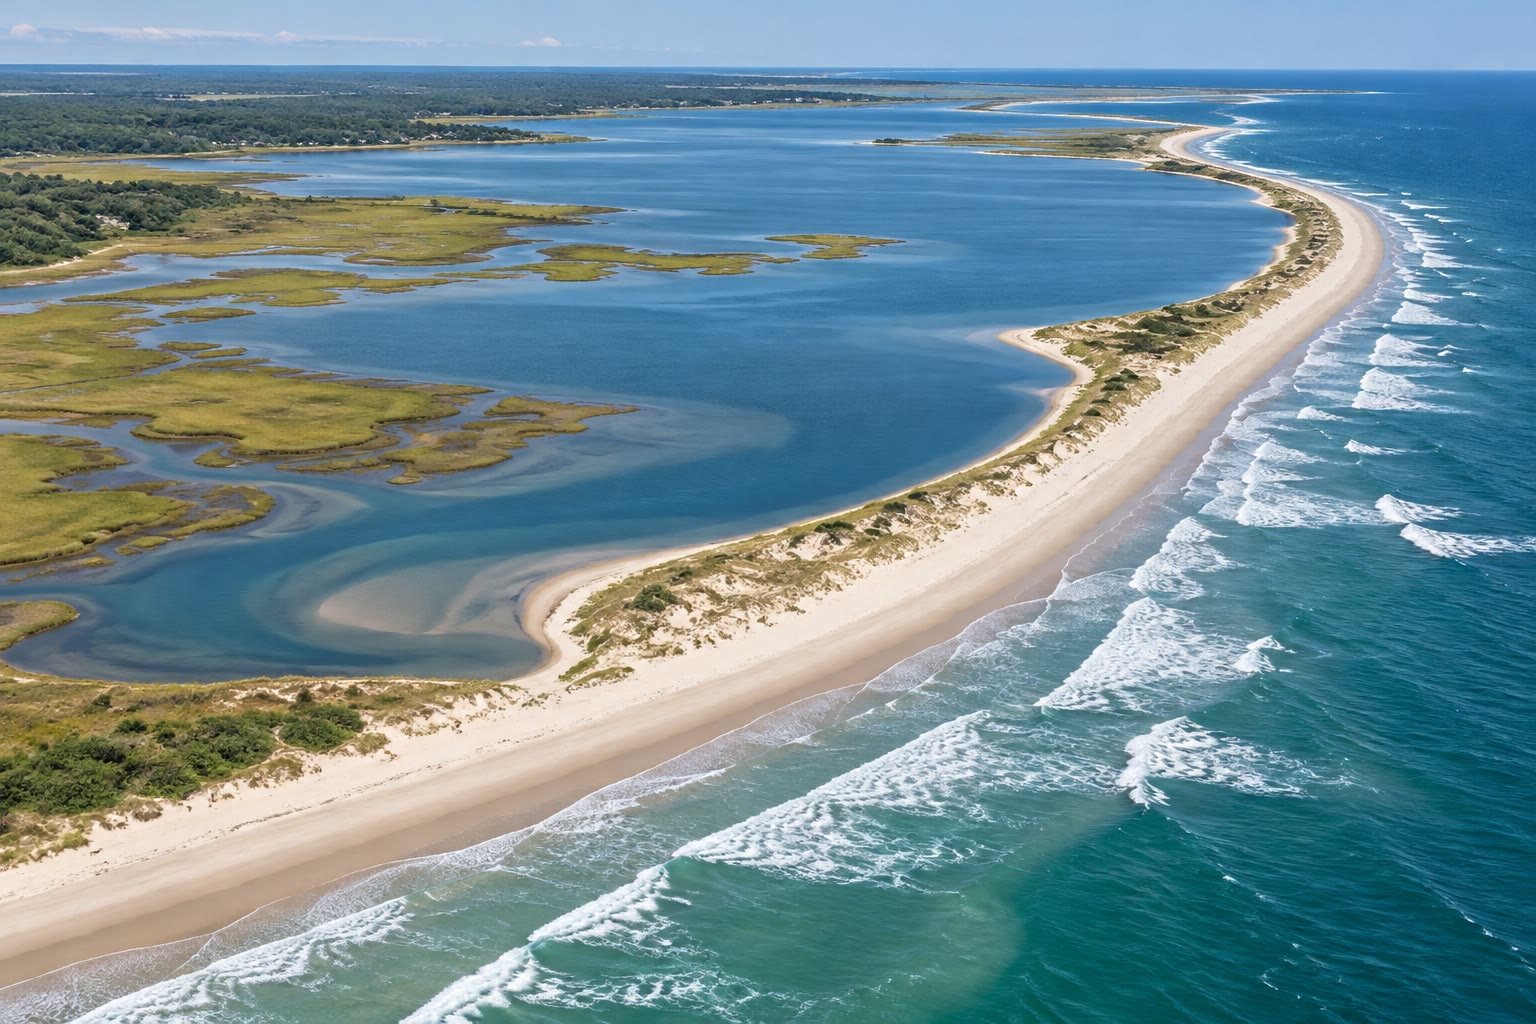
\includegraphics[width=\linewidth]{images/book1/ai/g9-spit-aerial.jpg}
\end{minipage}\hfill
\begin{minipage}[c]{0.46\linewidth}\raggedright
{\small \omterm{def:g9:landforms:beach}{Lidah pasir} yang melintangi mulut sebuah teluk, dilihat dari
pesawat terbang yang terbang rendah (ilustrasi, bukan tempat yang nyata).
Ombak pecah di \omterm{def:g9:landforms:beach}{gisiknya} yang menghadap \omterm{def:g2:water-on-earth:ocean}{laut}; di belakangnya terdapat air
yang tenang dan rawa asin.}
\end{minipage}
\label{fig:g9:landforms:spit-ai}
\end{omfigure}

\section{Bentuk lahan buatan pelarutan: karst}

Air \omterm{def:g4:clouds-rain-snow:precipitation}{hujan} bukanlah air murni. Ketika jatuh melalui udara lalu meresap ke
dalam tanah, air \omterm{def:g4:clouds-rain-snow:precipitation}{hujan} menyerap karbon dioksida, yang membuatnya sedikit
asam. Asam lemah ini melakukan secara perlahan apa yang dilakukan setetes
asam encer dengan cepat pada sepotong batu kapur: melarutkan \omterm{def:g3:stones-pebbles-sand:rock}{batuan} itu.
Batu kapur penuh retakan, di sepanjang lapisan-lapisannya maupun
melintanginya. Air merembes turun melalui retakan itu dan melebarkannya,
milimeter demi milimeter, selama ribuan tahun.
% ledger: usgs:sinkholes, nps:karst

\begin{definition}[Karst, gua, dan dolina]\label{def:g9:landforms:karst}
Yang disebut \emph{karst}\index{karst} adalah \omterm{def:g1:landscapes-around-us:landscape}{bentang alam} yang dibentuk
oleh air yang melarutkan \omterm{def:g3:stones-pebbles-sand:rock}{batuan} yang mudah larut, paling sering batu
kapur. Di sana, \omterm{def:g1:landscapes-around-us:water}{sungai-sungai} cenderung menghilang ke bawah tanah lalu
muncul kembali sebagai \omterm{def:g6:water-underground:spring}{mata air}. Yang disebut \emph{gua}\index{gua} adalah
ruang alami di bawah tanah yang cukup besar untuk dimasuki orang, yang
terlarut di sepanjang retakan \omterm{def:g3:stones-pebbles-sand:rock}{batuan}. Yang disebut
\emph{dolina}\index{dolina} adalah cekungan atau lubang di permukaan
tanah, yang terbentuk di tempat \omterm{def:g3:stones-pebbles-sand:rock}{batuan} di bawahnya larut atau di tempat
atap sebuah gua runtuh.
\end{definition}
% ledger: nps:karst, usgs:sinkholes

\begin{omfigure}
\begin{tikzpicture}[x=0.9cm, y=0.9cm, font=\footnotesize, >={Stealth[length=2mm]}]
  \pic (B) at (0,0) {blockdiagram={10}{4}{4}};
  % top face: grassland
  \fill[green!25!black!18] (B-ftl) -- (B-ftr) -- (B-btr) -- (B-btl) -- cycle;
  % right face
  \fill[omLithLime!70] (B-fbr) -- (B-bbr) -- (B-btr) -- (B-ftr) -- cycle;
  % front face: limestone layers
  \fill[omLithLime] (B-fbl) rectangle (B-ftr);
  \foreach \y in {0.8,1.6,2.4,3.2} \draw[black!35] (0,\y) -- (10,\y);
  \foreach \x/\y in {1.2/0.8, 3.1/1.6, 4.6/0, 6.8/2.4, 8.3/0.8, 2.2/2.4, 9.1/2.4, 5.6/3.2}
    \draw[black!35] (\x,\y) -- ++(0,0.8);
  % soil
  \fill[brown!45] (0,3.8) rectangle (10,4);
  % sinkhole on the top face and in the front face
  \fill[green!25!black!35] (3.0,4.45) ellipse (0.7 and 0.22);
  \fill[white] (2.3,4) -- (3.7,4) -- (3.25,3.45) -- (2.75,3.45) -- cycle;
  \fill[green!25!black!30] (2.3,4) -- (3.7,4) -- (3.25,3.45) -- (2.75,3.45) -- cycle;
  \draw[black!60] (2.3,4) -- (2.75,3.45) -- (3.25,3.45) -- (3.7,4);
  % shaft from sinkhole to cave
  \fill[white] (2.85,3.45) -- (3.15,3.45) -- (3.35,2.0) -- (3.05,2.0) -- cycle;
  \draw[black!60] (2.85,3.45) -- (3.05,2.0) (3.15,3.45) -- (3.35,2.0);
  % cave
  \fill[white] (2.6,2.1) .. controls (3.5,2.35) and (5.5,2.3) .. (6.6,1.9)
     .. controls (7.4,1.6) and (7.6,1.2) .. (7.2,1.0)
     .. controls (6.0,0.85) and (4.0,1.0) .. (3.0,1.2)
     .. controls (2.3,1.35) and (2.1,1.9) .. (2.6,2.1) -- cycle;
  \draw[black!70] (2.6,2.1) .. controls (3.5,2.35) and (5.5,2.3) .. (6.6,1.9)
     .. controls (7.4,1.6) and (7.6,1.2) .. (7.2,1.0)
     .. controls (6.0,0.85) and (4.0,1.0) .. (3.0,1.2)
     .. controls (2.3,1.35) and (2.1,1.9) .. (2.6,2.1);
  % underground stream at the cave floor
  \fill[omRiver!60] (3.0,1.2) .. controls (4.0,1.0) and (6.0,0.85) .. (7.2,1.0) -- (7.1,1.12)
     .. controls (6.0,1.0) and (4.0,1.12) .. (3.1,1.3) -- cycle;
  % stalactites and stalagmites
  \foreach \x/\l in {4.2/0.35, 4.5/0.22, 4.9/0.4, 5.3/0.25, 5.8/0.3}
    \fill[black!45] (\x-0.07,2.22) -- (\x+0.06,2.22) -- (\x,2.22-\l) -- cycle;
  \foreach \x/\l in {4.9/0.3, 5.8/0.25}
    \fill[black!45] (\x-0.12,0.95) -- (\x+0.12,0.95) -- (\x,0.95+\l) -- cycle;
  % disappearing stream on the top face
  \draw[omRiver, line width=1.2pt] (7.4,4.85) .. controls (6.9,4.5) and (6.4,4.4) .. (6.0,4.25);
  \fill[black!70] (6.0,4.25) circle (0.07);
  \draw[omRiver, dashed, thick] (6.0,4.0) -- (6.4,2.1);
  % spring on the right face
  \draw[omRiver, line width=1.2pt, ->] (10.2,1.2) .. controls (10.8,1.1) and (11.2,0.7) .. (11.6,0.5);
  % rain with carbon dioxide
  \foreach \x in {0.6,1.2,1.8} \draw[->, omRiver] (\x,5.6) -- ++(-0.15,-0.7);
  \draw[->, omRiver, dashed] (1.0,3.9) -- (1.2,1.7);
  % outline
  \draw[black!70] (B-fbl) rectangle (B-ftr);
  \draw[black!70] (B-ftl) -- (B-btl) -- (B-btr) -- (B-ftr) (B-btr) -- (B-bbr) -- (B-fbr);
  % labels
  \node[anchor=south, align=center] at (1.2,5.6) {hujan menyerap karbon\\dioksida: sedikit asam};
  \node[anchor=east, align=right] at (-0.1,1.6) {air melebarkan\\retakan};
  \draw[black!70] (-0.05,1.6) -- (1.1,2.0);
  \node[anchor=south] at (3.0,5.2) {dolina};
  \draw[black!70] (3.0,5.2) -- (3.0,4.55);
  \node[anchor=south, align=center] at (7.6,5.3) {sungai kecil menghilang\\ke bawah tanah};
  \draw[black!70] (7.0,5.3) -- (6.1,4.35);
  \node[anchor=north, align=center] at (5.0,-0.1) {gua: stalaktit bergantung dari atap,\\stalagmit tumbuh dari lantai};
  \draw[black!70] (5.0,-0.1) -- (5.0,1.4);
  \node[anchor=west, align=left] at (11.6,0.6) {mata air};
  \node[anchor=west] at (11.9,3.4) {batu kapur};
\end{tikzpicture}

{\small \omterm{def:g1:landscapes-around-us:landscape}{Bentang alam} \omterm{def:g9:landforms:karst}{karst} (sketsa, tidak berskala). Air yang sedikit asam
merembes melalui retakan batu kapur dan melebarkannya; \omterm{def:g1:landscapes-around-us:water}{sungai} bawah
tanah melubangi \omterm{def:g9:landforms:karst}{gua}; atap \omterm{def:g9:landforms:karst}{gua} runtuh dan membuka \omterm{def:g9:landforms:karst}{dolina}; sebuah \omterm{def:g1:landscapes-around-us:water}{sungai}
kecil menghilang ke dalam lubang lalu muncul kembali sebagai \omterm{def:g6:water-underground:spring}{mata air} di
tempat yang lebih rendah.}
% ledger: nps:karst, usgs:sinkholes, nps:speleothems
\label{fig:g9:landforms:karst}
\end{omfigure}

Di dalam \omterm{def:g9:landforms:karst}{gua}, pelarutan dapat berjalan terbalik. Setetes air yang merembes
dari atap membawa batu kapur yang terlarut. Ketika bertemu dengan udara
\omterm{def:g9:landforms:karst}{gua}, tetes itu melepaskan sebagian karbon dioksidanya, dan selaput tipis
kalsit keluar dari air di sekeliling tetes itu. Tetes demi tetes, sebuah
tabung berongga tumbuh dari atap, lalu menebal menjadi
\emph{stalaktit}\index{stalaktit}, yang bergantung seperti es runcing.
Di tempat tetes-tetes itu jatuh, sisa kalsitnya membangun
\emph{stalagmit}\index{stalagmit} yang tumbuh dari lantai. Ketika keduanya
bertemu, terbentuklah sebuah tiang.
% ledger: nps:speleothems

\begin{omfigure}
\begin{minipage}[c]{0.5\linewidth}\centering
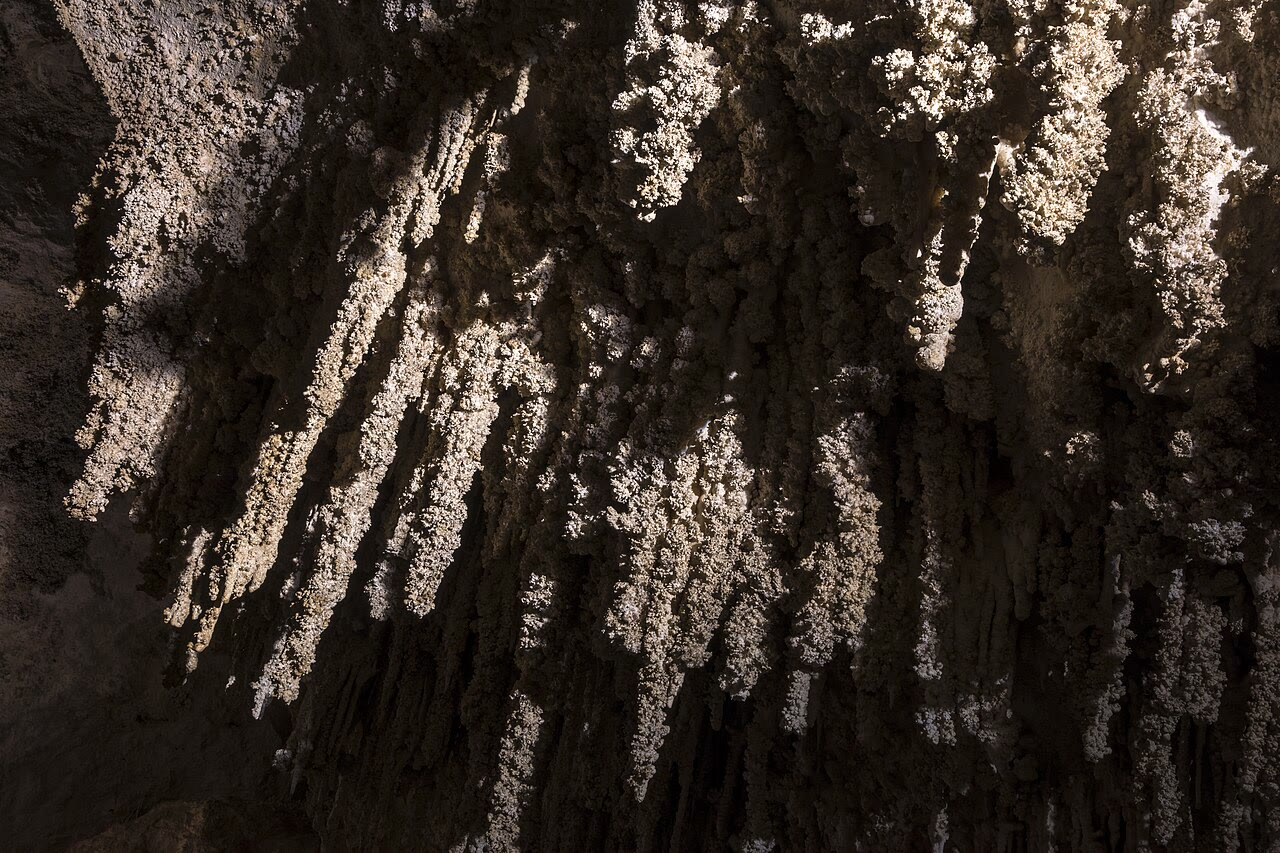
\includegraphics[width=\linewidth]{images/book1/g9-stalactites.jpg}
\end{minipage}\hfill
\begin{minipage}[c]{0.46\linewidth}\raggedright
{\small Stalaktit yang bergantung di bawah sebuah bongkah \omterm{def:g3:stones-pebbles-sand:rock}{batuan} besar di
Carlsbad Cavern, New Mexico, sebuah \omterm{def:g9:landforms:karst}{gua} yang terlarut di dalam batu
kapur. Setiap stalaktit tumbuh tetes demi tetes dari air yang merembes
melalui \omterm{def:g3:stones-pebbles-sand:rock}{batuan} di atasnya. National Park Service, 2018 (domain publik,
melalui Wikimedia Commons).}
\end{minipage}
% ledger: commons:carlsbad-stalactites, nps:speleothems
\label{fig:g9:landforms:stalactites}
\end{omfigure}

Daerah \omterm{def:g9:landforms:karst}{karst} menyimpan banyak air di bawah tanah, tetapi air itu mengalir
cepat melalui retakan-retakan yang terbuka dan hampir tidak tersaring:
apa pun yang tumpah di permukaan tanah dapat dengan cepat mencapai \omterm{def:g6:water-underground:spring}{mata
air}. Selain itu, di tempat \omterm{def:g3:stones-pebbles-sand:rock}{batuan} di bawahnya telah larut, tanah dapat
amblas atau runtuh: di tempat permukiman, \omterm{def:g9:landforms:karst}{dolina} yang tiba-tiba terbuka
dapat menelan jalan dan rumah.
% ledger: nps:karst, usgs:sinkholes

\section{Membaca bentang alam}

Setiap \omterm{def:g1:landscapes-around-us:landform}{bentuk lahan} adalah petunjuk. Bentuknya menunjukkan tenaga mana
yang membuatnya; tenaga itu menunjukkan proses mana yang bekerja, \omterm{def:g5:water-shapes-the-land:erosion}{erosi}
atau \omterm{def:g5:water-shapes-the-land:deposition}{pengendapan}; dan proses itu sering menunjukkan sesuatu tentang
\omterm{def:g3:stones-pebbles-sand:rock}{batuan} atau bahan lepas di bawahnya.

\begin{method}[Membaca bentuk lahan]
\begin{enumerate}
  \item \textbf{Bentuk.} Uraikan \omterm{def:g1:landscapes-around-us:landform}{bentuk lahan} itu: pematang, cekungan,
        permukaan yang curam, paparan yang datar; ukurannya; ke arah mana
        bentuk itu menghadap.
  \item \textbf{Tenaga dan proses.} Tentukan tenaga mana yang membuatnya
        (\omterm{def:g1:landscapes-around-us:water}{sungai}, es, angin, \omterm{def:g2:water-on-earth:ocean}{laut}, air yang melarutkan) dan apakah bentuk itu
        dipahat (\omterm{def:g5:water-shapes-the-land:erosion}{erosi}) atau dibangun (\omterm{def:g5:water-shapes-the-land:deposition}{pengendapan}).
  \item \textbf{Bahan.} Katakan dari apa bentuk itu tersusun, atau \omterm{def:g3:stones-pebbles-sand:rock}{batuan}
        apa yang kemungkinan ada di bawahnya: \omterm{def:g3:stones-pebbles-sand:sand}{pasir} lepas, \omterm{def:g3:stones-pebbles-sand:pebble}{kerikil}, batu
        kapur, \omterm{def:g3:stones-pebbles-sand:rock}{batuan} keras atau lunak.
\end{enumerate}
\end{method}

\begin{center}
{\small
\begin{tabular}{|>{\raggedright\arraybackslash}p{4.6cm}|>{\raggedright\arraybackslash}p{2.6cm}|>{\raggedright\arraybackslash}p{2.2cm}|>{\raggedright\arraybackslash}p{2.6cm}|}
\hline
bentuk & tenaga & proses & bahan \\
\hline
\omterm{def:g1:landscapes-around-us:landform}{bukit-bukit} \omterm{def:g3:stones-pebbles-sand:sand}{pasir} berbentuk bulan sabit & angin & \omterm{def:g5:water-shapes-the-land:deposition}{pengendapan} & \omterm{def:g3:stones-pebbles-sand:sand}{pasir} lepas \\
permukaan \omterm{def:g3:stones-pebbles-sand:rock}{batuan} tegak di atas paparan \omterm{def:g3:stones-pebbles-sand:rock}{batuan} yang datar & \omterm{def:g2:water-on-earth:ocean}{laut} & \omterm{def:g5:water-shapes-the-land:erosion}{erosi} & \omterm{def:g3:stones-pebbles-sand:rock}{batuan} (\omterm{def:g3:stones-pebbles-sand:rock}{batuan} lunak mundur dengan cepat) \\
pematang \omterm{def:g3:stones-pebbles-sand:sand}{pasir} yang sempit melintangi teluk & \omterm{def:g2:water-on-earth:ocean}{laut} (\omterm{def:g9:landforms:beach}{hanyutan sepanjang pantai}) & \omterm{def:g5:water-shapes-the-land:deposition}{pengendapan} & \omterm{def:g3:stones-pebbles-sand:sand}{pasir} atau \omterm{def:g3:stones-pebbles-sand:pebble}{kerikil} \\
cekungan-cekungan di ladang, \omterm{def:g1:landscapes-around-us:water}{sungai} kecil yang menghilang & air yang melarutkan & pelarutan & batu kapur \\
\omterm{def:g8:ice-on-earth:glacial-landforms}{lembah berbentuk U} & es & \omterm{def:g5:water-shapes-the-land:erosion}{erosi} & \omterm{def:g3:stones-pebbles-sand:rock}{batuan} apa pun \\
kipas \omterm{def:g3:stones-pebbles-sand:sand}{lumpur} di muara \omterm{def:g1:landscapes-around-us:water}{sungai} & \omterm{def:g1:landscapes-around-us:water}{sungai} & \omterm{def:g5:water-shapes-the-land:deposition}{pengendapan} & \omterm{def:g3:stones-pebbles-sand:sand}{lumpur} dan \omterm{def:g3:stones-pebbles-sand:sand}{pasir} \\
\hline
\end{tabular}}
\end{center}

\begin{example}[Berjalan-jalan di sebuah dataran tinggi]
Di sebuah dataran tinggi berumput yang tinggi, tidak ada \omterm{def:g1:landscapes-around-us:water}{sungai} sama
sekali, walaupun \omterm{def:g4:clouds-rain-snow:precipitation}{hujan} sering turun. Ladang-ladangnya bertaburan cekungan
bundar selebar beberapa meter, dan di \omterm{def:g1:landscapes-around-us:landform}{lembah} di bawahnya sebuah \omterm{def:g6:water-underground:spring}{mata air}
yang deras memancar dari kaki sebuah dinding \omterm{def:g3:stones-pebbles-sand:rock}{batuan}. \emph{Bentuk}:
cekungan, tidak ada \omterm{def:g1:landscapes-around-us:water}{sungai} di permukaan, \omterm{def:g6:water-underground:spring}{mata air} di tempat yang lebih
rendah. \emph{Tenaga dan proses}: air yang melarutkan \omterm{def:g3:stones-pebbles-sand:rock}{batuan} dan mengalir
di bawah tanah. \emph{Bahan}: dataran tinggi itu kemungkinan besar batu
kapur, dan cekungan-cekungannya adalah \omterm{def:g9:landforms:karst}{dolina}. Setetes asam encer pada
sepotong \omterm{def:g3:stones-pebbles-sand:rock}{batuan} yang lepas, yang diteteskan oleh guru, akan berbuih.
\end{example}
% ledger: nps:karst, usgs:sinkholes

\section{Latihan}

\begin{exercise}[$\star$]\label{exo:g9:landforms:1}
Tenaga mana yang membuat setiap \omterm{def:g1:landscapes-around-us:landform}{bentuk lahan} ini: angin, \omterm{def:g2:water-on-earth:ocean}{laut}, \omterm{def:g1:landscapes-around-us:water}{sungai}, es,
atau air yang melarutkan \omterm{def:g3:stones-pebbles-sand:rock}{batuan}? (a) \omterm{def:g1:landscapes-around-us:landform}{Bukit} \omterm{def:g3:stones-pebbles-sand:sand}{pasir} berbentuk bulan sabit di
\omterm{def:g5:weather-and-climate:desert}{gurun}. (b) \omterm{def:g9:landforms:karst}{Gua} yang penuh stalaktit. (c) Pematang \omterm{def:g3:stones-pebbles-sand:pebble}{kerikil} yang panjang
melintangi mulut sebuah teluk. (d) \omterm{def:g8:ice-on-earth:glacial-landforms}{Lembah berbentuk U} dengan \omterm{def:g8:ice-on-earth:glacial-landforms}{morena} di
ujungnya. (e) Dinding kapur yang tegak dengan paparan \omterm{def:g3:stones-pebbles-sand:rock}{batuan} yang datar di
kakinya. (f) \omterm{def:g5:water-shapes-the-land:delta}{Delta}.
\end{exercise}

\begin{exercise}[$\star$]\label{exo:g9:landforms:2}
Berikan istilah untuk setiap uraian. (a) Naiknya \omterm{def:g3:stones-pebbles-sand:rock}{batuan} dan permukaan
tanah suatu wilayah secara perlahan. (b) Sisi \omterm{def:g9:landforms:dune}{gumuk pasir} yang curam, yang
membelakangi angin. (c) Lubang di permukaan tanah yang terbentuk di tempat
\omterm{def:g3:stones-pebbles-sand:rock}{batuan} di bawahnya larut atau atap \omterm{def:g9:landforms:karst}{gua} runtuh. (d) Gerakan \omterm{def:g3:stones-pebbles-sand:sand}{pasir} dan
\omterm{def:g3:stones-pebbles-sand:pebble}{kerikil} di sepanjang tepi \omterm{def:g2:water-on-earth:ocean}{laut}. (e) \omterm{def:g1:landscapes-around-us:landscape}{Bentang alam} yang dibentuk oleh air
yang melarutkan batu kapur.
\end{exercise}

\begin{exercise}[$\star$]\label{exo:g9:landforms:3}
Benar atau salah? Perbaiki kalimat yang salah. (a) Tanduk \omterm{def:g9:landforms:dune}{gumuk pasir}
bulan sabit menunjuk ke arah datangnya angin. (b) Lereng \omterm{def:g9:landforms:dune}{gumuk pasir} yang
menghadap angin landai. (c) \omterm{def:g9:landforms:dune}{Gumuk pasir} bergerak karena angin
mengangkatnya sekaligus. (d) \omterm{def:g9:landforms:dune}{Gumuk pasir} lebih mudah terbentuk di tempat
yang sedikit tumbuhannya.
\end{exercise}

\begin{exercise}[$\star$]\label{exo:g9:landforms:4}
Urutkan langkah-langkah mundurnya \omterm{def:g9:landforms:cliff}{tebing} \omterm{def:g2:water-on-earth:ocean}{laut} ini. (a) Ombak memecah
bongkah-bongkah yang jatuh dan mengangkutnya pergi. (b) Ombak memahat
takik di kaki \omterm{def:g9:landforms:cliff}{tebing}. (c) Permukaan \omterm{def:g9:landforms:cliff}{tebing} sekarang berdiri lebih jauh ke
arah daratan, dan \omterm{def:g1:landscapes-around-us:landform}{dataran} yang datar di depannya sedikit lebih lebar.
(d) \omterm{def:g3:stones-pebbles-sand:rock}{Batuan} di atas takik menggantung. (e) Bagian yang menggantung runtuh.
\end{exercise}

\begin{exercise}[$\star\star$]\label{exo:g9:landforms:5}
% ledger: nps:whsa-migration (6 and 3 m a year)
Dilihat dari pesawat terbang, \omterm{def:g9:landforms:dune}{gumuk-gumuk} \omterm{def:g3:stones-pebbles-sand:sand}{pasir} bulan sabit di sebuah
\omterm{def:g5:weather-and-climate:desert}{gurun} semuanya mempunyai tanduk yang menunjuk ke timur. (a) Dari arah mana
angin bertiup? (b) Di sisi mana \omterm{def:g9:landforms:dune}{lereng luncur} setiap \omterm{def:g9:landforms:dune}{gumuk}? (c) Sebuah
jalan membentang \qty{60}{m} di sebelah timur salah satu \omterm{def:g9:landforms:dune}{gumuk}. \omterm{def:g9:landforms:dune}{Gumuk} itu
bergerak \qty{6}{m} setahun. Dalam berapa tahun kakinya akan mencapai
jalan itu? (d) Sebuah \omterm{def:g9:landforms:dune}{gumuk} yang lebih besar hanya bergerak \qty{3}{m}
setahun. Mengapa \omterm{def:g9:landforms:dune}{gumuk} yang lebih besar bergerak lebih lambat?
\end{exercise}

\begin{exercise}[$\star\star$]\label{exo:g9:landforms:6}
% ledger: sdnp:birling, nt:birling-2014
\omterm{def:g9:landforms:cliff}{Tebing} kapur di sebuah \omterm{def:g1:landscapes-around-us:water}{pesisir} mundur sampai sekitar \qty{1}{m} setahun.
Pada musim dingin tahun 2014, \omterm{def:g9:landforms:cliff}{tebing} itu kehilangan sebanyak yang biasanya
hilang dalam tujuh tahun, hanya dalam dua bulan. (a) Dengan \qty{1}{m}
setahun, berapa yang hilang dalam tujuh tahun? (b) Dua bulan adalah
pecahan berapa dari satu tahun? (c) Berapa kali lebih cepat daripada
biasanya \omterm{def:g9:landforms:cliff}{tebing} itu mundur selama dua bulan itu? (d) Jelaskan, dengan
memakai takik dan bagian yang menggantung, mengapa \omterm{def:g9:landforms:cliff}{tebing} mundur dengan
lompatan alih-alih secara mulus.
\end{exercise}

\begin{exercise}[$\star\star$]\label{exo:g9:landforms:7}
Sebuah \omterm{def:g1:landscapes-around-us:water}{pesisir} yang lurus membentang dari barat ke timur, dengan \omterm{def:g2:water-on-earth:ocean}{laut} di
sebelah selatan. Ombak datang dari barat daya. (a) Ke arah mana \omterm{def:g9:landforms:beach}{hanyutan
sepanjang pantai} membawa \omterm{def:g3:stones-pebbles-sand:sand}{pasir}? (b) Gambarlah lintasan zigzag sebuah
\omterm{def:g3:stones-pebbles-sand:pebble}{kerikil} selama tiga kali ombak, dengan memberi keterangan gerakan naik ke
\omterm{def:g9:landforms:beach}{gisik} dan gerakan kembali turun. (c) Di ujung timurnya, \omterm{def:g1:landscapes-around-us:water}{pesisir} itu
berbelok ke utara membentuk teluk. \omterm{def:g1:landscapes-around-us:landform}{Bentuk lahan} apa yang kemungkinan
tumbuh di sana? (d) Mengapa \omterm{def:g3:stones-pebbles-sand:sand}{lumpur} mengendap di belakangnya?
\end{exercise}

\begin{exercise}[$\star\star$]\label{exo:g9:landforms:8}
(a) Apa yang membuat air \omterm{def:g4:clouds-rain-snow:precipitation}{hujan} sedikit asam? (b) Mengapa ada \omterm{def:g9:landforms:karst}{gua} di batu
kapur tetapi hampir tidak ada di granit? (c) Mengapa \omterm{def:g9:landforms:karst}{gua} mengikuti
retakan dan lapisan \omterm{def:g3:stones-pebbles-sand:rock}{batuan}? (d) Berikan dua cara terbentuknya \omterm{def:g9:landforms:karst}{dolina}.
\end{exercise}

\begin{exercise}[$\star\star$]\label{exo:g9:landforms:9}
(a) Jelaskan mengapa kalsit keluar dari setetes air yang menggantung di
atap \omterm{def:g9:landforms:karst}{gua}. (b) Mengapa stalagmit tidak mempunyai tabung berongga di
dalamnya, tidak seperti stalaktit yang masih muda? (c) Misalkan sebuah
stalaktit tumbuh \qty{0.1}{mm} setahun (laju rekaan: laju yang sebenarnya
sangat beragam). Berapa tahun yang diperlukannya untuk tumbuh
\qty{30}{cm}? Tuliskan jawabannya dalam notasi ilmiah.
\end{exercise}

\begin{exercise}[$\star\star$]\label{exo:g9:landforms:10}
% ledger: usgs:himalaya, sdnp:birling
\omterm{def:g1:landscapes-around-us:landform}{Dataran} Tinggi Tibet naik sekitar \qty{4600}{m} dalam sekitar 10~juta
tahun. (a) Hitunglah rata-rata \omterm{def:g9:landforms:uplift}{pengangkatannya} dalam meter per tahun,
dalam notasi ilmiah, lalu dalam milimeter per tahun. (b) Misalkan \omterm{def:g5:water-shapes-the-land:erosion}{erosi}
mengikis \qty{0.2}{mm} setahun dari dataran tinggi itu (angka rekaan).
Berapa besar dataran tinggi itu naik setiap tahun? (c) \omterm{def:g9:landforms:cliff}{Tebing} kapur mundur
sekitar \qty{1}{m} setahun. Berapa kali lebih cepat itu dibandingkan
dengan \omterm{def:g9:landforms:uplift}{pengangkatan} pada (a)? (d) Mengapa \omterm{def:g9:landforms:uplift}{pengangkatan} yang lambat tetap
dapat membangun dataran tinggi yang tinggi?
\end{exercise}

\begin{exercise}[$\star\star\star$]\label{exo:g9:landforms:11}
Bacalah setiap \omterm{def:g1:landscapes-around-us:landscape}{bentang alam} dengan metode bab ini (bentuk, tenaga dan
proses, bahan). (a) Di sebuah negeri yang kering, deretan panjang \omterm{def:g1:landscapes-around-us:landform}{bukit}
\omterm{def:g3:stones-pebbles-sand:sand}{pasir}, masing-masing berbentuk bulan sabit, dengan sisi curam yang
menghadap ke tenggara. (b) Di kaki sebuah \omterm{def:g9:landforms:cliff}{tebing} putih, paparan \omterm{def:g3:stones-pebbles-sand:rock}{batuan}
yang datar dan tertutup rumput \omterm{def:g2:water-on-earth:ocean}{laut} muncul saat air surut. (c) Di sebuah
dataran tinggi yang luas dengan \omterm{def:g3:stones-pebbles-sand:rock}{batuan} berwarna pucat, sebuah \omterm{def:g1:landscapes-around-us:water}{sungai}
kecil mengalir melintasi ladang lalu menghilang ke dalam lubang; sebuah
\omterm{def:g6:water-underground:spring}{mata air} memancar dari sisi \omterm{def:g1:landscapes-around-us:landform}{lembah} yang berjarak \qty{2}{km}.
\end{exercise}

\begin{exercise}[$\star\star\star$]\label{exo:g9:landforms:12}
% ledger: nps:whsa-migration, nmt:barchan, nps:aeolian
Di sebuah padang \omterm{def:g9:landforms:dune}{gumuk pasir}, \omterm{def:g9:landforms:dune}{gumuk-gumuk} kecil di tepi hulu anginnya
bergerak sampai \qty{6}{m} setahun; sedikit lebih jauh, \omterm{def:g9:landforms:dune}{gumuk-gumuk} yang
tingginya 6 sampai \qty{10}{m} bergerak sekitar \qty{3}{m} setahun. Sebuah
jalan setapak melintasi padang itu \qty{45}{m} searah angin dari sebuah
\omterm{def:g9:landforms:dune}{gumuk} dari setiap jenis. (a) Setelah berapa tahun setiap \omterm{def:g9:landforms:dune}{gumuk} mencapai
jalan setapak itu? (b) \omterm{def:g9:landforms:dune}{Gumuk pasir} yang didorong angin kencang dapat
berpindah lebih dari \qty{100}{m} dalam setahun. Berapa lama \omterm{def:g9:landforms:dune}{gumuk} seperti
itu akan menempuh jarak yang sama? (c) Sebutkan satu cara untuk
memperlambat \omterm{def:g9:landforms:dune}{gumuk pasir}, dan jelaskan cara kerjanya.
\end{exercise}

\section{Soal: Tebing dan jalan pesisir}

\begin{problem}[{Soal akhir pekan --- sebuah jalan pesisir membentang di
belakang tebing kapur yang sedang mundur; jawaban terakhirnya adalah
tahun ketika tepi tebing akan mencapai jalan itu dengan laju yang
terukur}]
\label{pb:g9:landforms:1}
% ledger: (invented region: exercise data, figdata/grade-9/cliff_retreat.py; the rate is kept within sdnp:birling, the storm winter recalls nt:birling-2014)
Sebuah jalan \omterm{def:g1:landscapes-around-us:water}{pesisir} membentang di sepanjang puncak \omterm{def:g9:landforms:cliff}{tebing} kapur. Setiap
beberapa tahun, sebuah tim survei mengukur jarak dari jalan ke tepi \omterm{def:g9:landforms:cliff}{tebing}
di sepanjang garis yang sama, dari penanda-penanda tetap yang dipasang
jauh dari tepi, tidak pernah di tepi itu sendiri. Inilah hasil
pengukurannya.

\begin{center}
{\small
\begin{tabular}{|l|c|c|c|c|c|c|c|}
\hline
tahun & 2004 & 2008 & 2012 & 2014 & 2016 & 2020 & 2024 \\
\hline
jarak dari jalan ke tepi \omterm{def:g9:landforms:cliff}{tebing} (m) & 46.0 & 43.1 & 41.0 & 36.2 & 35.5 & 33.0 & 30.4 \\
\hline
\end{tabular}}
\end{center}

\noindent\textbf{Bagian I --- Hasil pengukuran.}\par\nopagebreak
\begin{enumerate}[beginpenalty=10000]
  \item Berapa meter tepi \omterm{def:g9:landforms:cliff}{tebing} bergeser mendekati jalan antara tahun
        2004 dan 2024?
  \item Hitunglah rata-rata laju mundurnya selama 20 tahun ini, dalam
        meter per tahun.
  \item Di antara dua survei yang mana tepi \omterm{def:g9:landforms:cliff}{tebing} mundur paling cepat?
        Hitunglah lajunya selama selang waktu itu.
  \item Berapa kali lebih cepat laju itu daripada rata-ratanya? Kemukakan
        dugaanmu tentang apa yang terjadi selama selang waktu itu.
\end{enumerate}

\begin{omfigure}
\begin{tikzpicture}
\begin{axis}[omrecord, width=11cm, height=4.6cm, xmin=2000, xmax=2070,
  ymin=0, ymax=50, xtick={2000,2010,...,2070}, ytick={0,10,...,50},
  x tick label style={/pgf/number format/1000 sep={}},
  xlabel={tahun}, ylabel={jarak ke jalan (m)}]
  \addplot[omWarm, thick, mark=*, mark size=1.8pt] table[x=year, y=dist_m] {figdata/out/grade-9-cliff_retreat.dat};
\end{axis}
\end{tikzpicture}

{\small Hasil survei: jarak dari jalan \omterm{def:g1:landscapes-around-us:water}{pesisir} ke tepi \omterm{def:g9:landforms:cliff}{tebing} (data
latihan).}
\label{fig:g9:landforms:survey}
\end{omfigure}

\noindent\textbf{Bagian II --- Lajunya.}\par\nopagebreak
\begin{enumerate}[resume, beginpenalty=10000]
  \item Tuliskan laju rata-ratanya dalam sentimeter per tahun, lalu dalam
        meter per abad.
  \item Di \omterm{def:g1:landscapes-around-us:water}{pesisir} kapur yang sebenarnya, \omterm{def:g9:landforms:cliff}{tebing} mundur sampai sekitar
        satu meter setahun. Apakah mundurnya \omterm{def:g9:landforms:cliff}{tebing} ini sebesar itu juga?
  \item Sebuah mercusuar di \omterm{def:g1:landscapes-around-us:water}{pesisir} semacam itu pernah dipindahkan
        \qty{17}{m} menjauhi tepi \omterm{def:g9:landforms:cliff}{tebing}. Dengan laju rata-rata \omterm{def:g9:landforms:cliff}{tebing} ini,
        \qty{17}{m} itu sama dengan mundurnya selama berapa tahun?
  \item Mengapa laju yang diukur selama 20 tahun merupakan pedoman yang
        lebih baik untuk masa depan daripada laju yang diukur selama dua
        tahun?
\end{enumerate}

\noindent\textbf{Bagian III --- Jalannya.}\par\nopagebreak
\begin{enumerate}[resume, beginpenalty=10000]
  \item Jalan itu harus dipindahkan sebelum tepi \omterm{def:g9:landforms:cliff}{tebing} mendekat sampai
        \qty{10}{m} darinya. Pada tahun berapa, dengan laju rata-rata, hal
        itu akan terjadi?
  \item Jika musim dingin yang lebih sering berbadai melipatduakan lajunya,
        pada tahun berapa tepi \omterm{def:g9:landforms:cliff}{tebing} akan mencapai jalan?
  \item Mengapa tim survei melakukan pengukurannya dari penanda yang
        dipasang jauh dari tepi \omterm{def:g9:landforms:cliff}{tebing}?
  \item Dengan laju rata-rata, pada tahun berapa tepi \omterm{def:g9:landforms:cliff}{tebing} akan mencapai
        jalan itu?
\end{enumerate}
\end{problem}
